\de{ĐỀ THI HỌC KỲ II NĂM HỌC 2022-2023}{THPT Nguyễn Hữu Tiến}

\begin{bt}%[0T7B2-1]%[Dự án đề kiểm tra HKII NH 22-23-Nhật Thiện]%[Trường NGUYỄN HỮU TIẾN]
	Lập bảng xét dấu và giải bất phương trình $2x^2-5x+2>0$.	
	\loigiai{
		Ta có bảng xét dấu
	\begin{center}
		\begin{tikzpicture}[scale=1, font=\footnotesize, line join=round, line cap=round, >=stealth]
		\tkzTabInit[nocadre=false,lgt=3,espcl=2.5,deltacl=0.6]
		{$x$ /1,$2x^2-5x+2$ /0.6}
		{$-\infty$,$\dfrac{1}{2}$, $2$,$+\infty$}
		\tkzTabLine{,+,0,-,0,+,}
		\end{tikzpicture}
	\end{center}
Dựa vào bảng xét dấu, $2x^2-5x+2>0\Leftrightarrow x<\dfrac{1}{2}$ hay $2<x$.
}
\end{bt}
\begin{bt}%[0T8B2-1]%[Dự án đề kiểm tra HKII NH 22-23-Nhật Thiện]%[Trường NGUYỄN HỮU TIẾN]
	\begin{enumerate}
		\item Có bao nhiêu cách sắp xếp $5$ học sinh thành một hàng dọc?
		\item Có bao nhiêu số tự nhiên gồm $4$ chữ số khác nhau được lập từ các chữ số $4$; $5$; $6$; $7$; $8$; $9$?
	\end{enumerate}
\loigiai{
	\begin{enumerate}
		\item Xếp $5$ học sinh vào một hàng dọc có $5!=120$ cách.
		\item Gọi $\overline{abcd}$ là số cần tìm.\\
		Chọn $4$ số khác nhau trong $6$ số đã cho và sắp xếp theo thứ tự có $\mathrm{A}_6^4=360$ số.
	\end{enumerate}
}
\end{bt}
\begin{bt}%[0T7B3-2]%[Dự án đề kiểm tra HKII NH 22-23-Nhật Thiện]%[Trường NGUYỄN HỮU TIẾN]
	Giải phương trình sau $3\sqrt{x^2+5x-23}=2x-3$.
	\loigiai{
	Ta có 
	\begin{eqnarray*}
		& &3\sqrt{x^2+5x-23}=2x-3\\
		&\Rightarrow& 9(x^2+5x-23)=(2x-3)^2\\
		&\Rightarrow& 5x^2+57x-216=0\\
		&\Rightarrow& \hoac{&x=-\dfrac{72}{5}\\&x=3.}
	\end{eqnarray*}
Thử lại, ta thấy $x=3$ thỏa mãn phương trình.\\
Vậy tập nghiệm của phương trình là $S=\{3\}$.
}
\end{bt}
\begin{bt}%[0T8K3-2]%[Dự án đề kiểm tra HKII NH 22-23-Nhật Thiện]%[Trường NGUYỄN HỮU TIẾN]
	\begin{enumerate}
		\item Tìm số hạng chứa $x^8$ trong khai triển của nhị thức $(2x^2+x)^5$.
		\item Tính tổng $S=\mathrm{C}_{2023}^0-2\mathrm{C}_{2023}^1+4\mathrm{C}_{2023}^2-8\mathrm{C}_{2023}^3+\ldots+2^{2022} \mathrm{C}_{2023}^{2022}-2^{2023}\mathrm{C}_{2023}^{2023}$.
	\end{enumerate}
\loigiai{
	\begin{enumerate}
		\item Khai triển của nhị thức 
		\begin{eqnarray*}
			& &(2x^2+x)^5\\
			&=&\mathrm{C}_5^0 (2x^2)^0 x^5+\mathrm{C}_5^1 (2x^2)^1 x^4+\mathrm{C}_5^2 (2x^2)^2 x^3+\mathrm{C}_5^3 (2x^2)^3 x^2+\mathrm{C}_5^4 (2x^2)^4 x^1+\mathrm{C}_5^5 (2x^2)^5 x^0\\
			&=&		x^5+10 x^6+40 x^7+80 x^8+80 x^9+32 x^{10}.
		\end{eqnarray*}
	\item Xét khai triển của nhị thức $(1-x)^{2023}$.\\
	Ta có 
	\begin{eqnarray*}
		& &(1-x)^{2023}\\
		&=&\mathrm{C}_{2023}^0 1^0 (-x)^{2023}+\mathrm{C}_{2023}^1 1^1 (-x)^{2022}+\ldots+\mathrm{C}_{2023}^{2022} 1^{2022} (-x)^1+\mathrm{C}_{2023}^{2023} 1^{2023} (-x)^0\\
		&=&-\mathrm{C}_{2023}^0 x^{2023}+\mathrm{C}_{2023}^1 x^{2022}+\ldots - \mathrm{C}_{2023}^{2022} x+\mathrm{C}_{2023}^{2023}\\
		&=&-\mathrm{C}_{2023}^{2023} x^{2023}+\mathrm{C}_{2023}^{2022} x^{2022} +\ldots - \mathrm{C}_{2023}^1 x+\mathrm{C}_{2023}^0. 
	\end{eqnarray*}
	Cho $x=2$ ta được
	\begin{eqnarray*}
		(1-2)^{2023}&=&-\mathrm{C}_{2023}^{2023} 2^{2023} +\mathrm{C}_{2023}^{2022} 2^{2022}+\ldots - \mathrm{C}_{2023}^1 2 +\mathrm{C}_{2023}^0\\
		\Leftrightarrow (-1)^{2023}&=&\mathrm{C}_{2023}^0-2 \mathrm{C}_{2023}^1+\ldots +\mathrm{C}_{2023}^{2022} 2^{2022}-\mathrm{C}_{2023}^{2023} 2^{2023}\\
		\Leftrightarrow S=-1.
	\end{eqnarray*}
	\end{enumerate}
}
\end{bt}
\begin{bt}%[0T0B2-2]%[Dự án đề kiểm tra HKII NH 22-23-Nhật Thiện]%[Trường NGUYỄN HỮU TIẾN]
	Trong đợt kiểm tra giữa HK2 vừa qua, thống kê kết quả điểm kiểm tra môn Toán của lớp 11B8 ta được kết quả như sau
	\begin{center}
		\begin{tabular}{|c|c|c|c|c|c|c|}
			\hline
			\textbf{Xếp loại điểm}& Kém & Yếu & Trung bình & Khá & Giỏi &\\
			\hline
			\textbf{Số lượng} & $4$& $6$ &$13$& $13$ & $11$ & $N=47$\\
			\hline
		\end{tabular}
	\end{center}
	Chọn ngẫu nhiên $3$ học sinh trong lớp 11B8, tính xác suất để cả $3$ học sinh được chọn \textbf{không có} bạn nào xếp loại điểm Yếu và cũng \textbf{không có} bạn nào xếp loại điểm Kém?
	\loigiai{
	Phép thử chọn ngẫu nhiên $3$ học sinh có không gian mẫu $\Omega$, suy ra $n(\Omega)=\mathrm{C}_{47}^3$.\\
	Gọi $A$ là biến cố ``không có bạn xếp loại điểm Yếu và cũng không có bạn xếp loại điểm Kém''.\\
	Suy ra $n(A)=\mathrm{C}_{47-4-6}^3=\mathrm{C}_{37}^3$.\\
	Vậy xác suất cần tìm là $\mathrm{P}(A)=\dfrac{n(A)}{n(\Omega)}=\dfrac{518}{1081}$.
}
\end{bt}

\begin{bt}%[0T8B2-1] %[Dự án đề kiểm tra HKII NH 22-23-TheHung Nguyên]%[Trường NGUYỄN HỮU TIẾN]
	Đội tuyển học sinh giỏi Toán của trường THPT Nguyễn Hữu Tiến gồm $15$ học sinh trong đó có $9$ bạn nam. Giáo viên hướng dẫn cần chọn ra $5$ học sinh để tham dự hội thảo Toán học. Hỏi có bao nhiêu cách chọn $5$ học sinh nói trên sao cho $5$ học sinh được chọn có cả nam và nữ?
	\loigiai{
		\begin{itemize}
			\item Số cách chọn $5$ học sinh bất kỳ là $\mathrm{C}_{15}^5$ cách.
			\item Số cách chọn $5$ học sinh nam có $\mathrm{C}_9^5$ cách.
			\item Số cách chọn $5$ học sinh nữ có $\mathrm{C}_6^5$ cách.
		\end{itemize}
	Vậy số cách chọn $5$ học sinh đi dự hội thao Toán có cả nam và nữ là $\mathrm{C}_{15}^5-\mathrm{C}_9^5-\mathrm{C}_6^5=2871$ cách.
	}
\end{bt}



\begin{bt}% [0T9B4-2]%[Dự án đề kiểm tra HKII NH 22-23-TheHung Nguyên]%[Trường NGUYỄN HỮU TIẾN]
	Trong mặt phẳng tọa độ $Oxy$, lập phương trình chính tắc của elip $(E)$ biết $(E)$ có một tiêu điểm là $F_1(-4; 0)$ và có độ dài trục lớn bằng $10$.
	\loigiai{Phương trình chính tắc của $(E)$ có dạng $(E)\colon \dfrac{x^2}{a^2}+\dfrac{y^2}{b^2}=1$ với $a>0$, $b>0$.\\
		Ta có 
		\begin{itemize}
		\item 	Độ dài trục lớn bằng $10$ nên $2a=10\Leftrightarrow a=5$.
		\item $F_1(-4; 0)\Rightarrow c=4$ mà $b^2=a^2-c^2=5^2-4^2=9$.
		\end{itemize}
	Vậy $(E)\colon \dfrac{x^2}{25}+\dfrac{y^2}{9}=1$.
	}
\end{bt}

\begin{bt}%[0T9B3-2]%[Dự án đề kiểm tra HKII NH 22-23-TheHung Nguyên]%[Trường NGUYỄN HỮU TIẾN]
	Trong mặt phẳng tọa độ $Oxy$, cho tam giác $ABC$ với tọa độ $3$ đỉnh là $A(-1; 0)$, $B(1; 4)$ và $C(1;-2)$. Viết phương trình đường tròn $(C)$ ngoại tiếp tam giác $ABC$.
	\loigiai{Phương trình đường tròn $(C)$ qua $A$, $B$, $C$ có dạng
		$x^2+y^2-2a x-2b y+c=0~\text{với}~\left(a^2+b^2-c>0\right)$.
		Ta có $A,B, C\in (C)$ nên ta có
		$$\heva{&(-1)^2+0^2-2a\cdot(-1)-2b\cdot0+c=0\\ &1^2+4^2-2a\cdot1-2b\cdot4+c=0\\ &1^2+(-2)^2+2a\cdot1-2b\cdot(-2)+c=0}\Leftrightarrow\heva{&2a+c=1\\ &-2a-8b+c=-17\\ &-2a+4b+c=-5}\Leftrightarrow \heva{&a=2\\ &b=1\\ &c=-5.}$$
	Vậy $(C)\colon x^2+y^2-4x-2y-5=0$.	
	}
\end{bt}


\begin{bt}%[0T9B2-6]%[Dự án đề kiểm tra HKII NH 22-23-TheHung Nguyên]%[Trường NGUYỄN HỮU TIẾN]
	Trong mặt phẳng tọa độ $Oxy$, cho tam giác $DEF$ vuông tại $D$ biết đỉnh $D(-1;-2)$. Hai trong ba cạnh của tam giác nằm trên $2$ đường thẳng $d_1\colon x+y-3=0$ và $d_2\colon 2x-y=0$. Tìm tọa độ các đỉnh $E$ và $F$.
	\loigiai{\immini{Ta có 
		\begin{itemize}
				\item $2\cdot (-1)-1\cdot (-2)=0$ nên $D(-1;-2)\in d_2$.
				\item $-1-2-3=-6\ne 0$ nên $D(-1;-2)\notin d_1$.
		\end{itemize}
	Khi đó $E, F\in d_1$ và $D, F\in d_2$.\\
	Do đó tọa độ điểm $F$ là nghiệm của hệ $\heva{& x+y=3 \\ & 2x-y=0}\Leftrightarrow\heva{& x=1 \\ & y=2.}$\\
	Suy ra $F(1;2)$ và $\overrightarrow{DF}=(-1;0)$.\\
	Gọi $E(a;3-a)\in d_1\Rightarrow \overrightarrow{DE}=(a+1;5-a)$.
}{\begin{tikzpicture}[scale=1, font=\footnotesize, line join=round, line cap=round, >=stealth]
				\draw [shorten <= -.7cm, shorten >= -.7cm](0,0)coordinate (D)--node[midway,above,sloped]{$d_2$}(3,0)coordinate (F);
				\draw [shorten <= -.7cm, shorten >= -.7cm](D)--(0,4)coordinate (E);
				\draw[shorten <= -.7cm, shorten >= -.7cm] (E)--node[midway,above,sloped]{$d_1$}(F);
				\foreach \y/\g in {D/-50,F/30,E/10}  \fill (\y) circle (1pt)+(\g:.5)node {$\y$};
				\pic[draw, angle radius=4mm] {right angle=E--D--F};
		\end{tikzpicture}}
	\noindent Ta có $\overrightarrow{DF}\perp \overrightarrow{DE}\Rightarrow \overrightarrow{DF}\cdot \overrightarrow{DE}=0\Rightarrow -1\cdot (1+a)+0\cdot (5-a)=0\Leftrightarrow a=-1$. Suy ra $E(-1;4)$.	\\
	Vậy $F(1;2)$, $E(-1;4)$.		
	}
\end{bt}


